\documentclass[border=0pt, tikz]{standalone}
\usepackage{pgfplots}
\pgfplotsset{compat=1.16}
\usetikzlibrary{calc}

%z-buffer is not good

\begin{document}

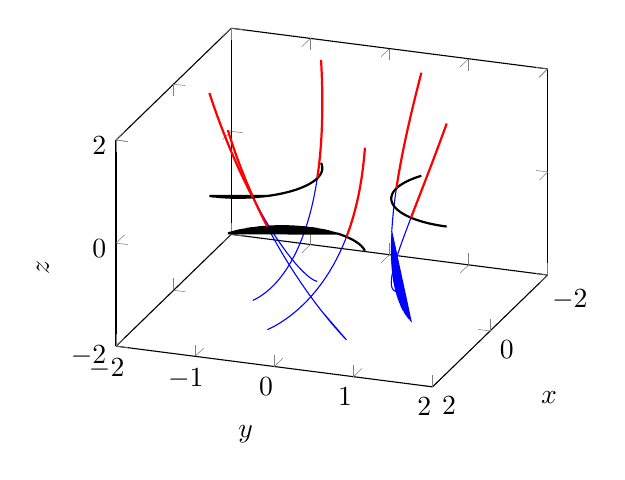
\begin{tikzpicture}
\begin{axis}%
[ scale=0.8
, view={110}{30} % {rotation angle}{elevation angle}
, z buffer=sort
, xlabel=$x$
, ylabel=$y$
, zlabel=$z$
, zmin=-2
, zmax=2
, xmin=-2
, xmax=2
, ymin=-2
, ymax=2
, declare function={
        s(\t) = (\t+30)/90;
    }
]

%% Parabola and cubic shadow curves
%\addplot3%
%[ samples=40
%, samples y=0
%, thick 
%, cyan 
%, domain=-2:2
%, variable=\t
%] ({t},{t^2},{-8});
%
%\addplot3%
%[ samples=40
%, samples y=0
%, thick
%, red 
%, domain=-2:2
%, variable=\t
%] ({t},{-1},{t^3});

%  Lines
%  (pgfplots cannot handle a \foreach commands inside the {axis} environment, so the draw commands need to have the foreach inside of them. See also pgfplotsinvokeforeach._

%\draw [cyan] foreach \a in {-2,-1.9,...,2} {
%({\a}, {(\a)^2}, {(\a)^3}) --  ({\a}, {(\a)^2}, -8)
%};
%
%\draw [black, thick]  {
%(-2,0,-2) -- (2, 0, -2) -- (2,0,2) -- (-2,0,2) -- cycle
%};

%\addplot3[
%    fill=gray!20,
%    draw=black,
%    thick,
%]
%coordinates {
%(-2,0,-2)
%(2,0,-2)
%(2,0,2)
%(-2,0,2)
%(-2,0,-2)
%};

% Twisted cubic
\foreach \k in {0,1,2}
{


\addplot3%
[ samples=100
, samples y=0
%, thick
, blue
, domain=-30:30
, variable=\t
] 
({sin (t-90+120*\k)+sqrt(3)*cos(120*\k)},{cos (t-90+120*\k)-sqrt(3)*sin(120*\k)},{3*s(-t)^2+s(-t)-2});

\addplot3%
[ samples=100
, samples y=0
%, thick
, blue
, domain=-30:30
, variable=\t
] 
({sin (t-90+120*\k)+sqrt(3)*cos(120*\k)},{cos (t-90+120*\k)-sqrt(3)*sin(120*\k)},{3*s(t)^2+s(t)-2});

}

\foreach \k in {0,1,2}
{


\addplot3%
[ samples=100
, samples y=0
, thick
, black 
, domain=-60:60
, variable=\t
] 
({sin (t-90+120*\k)+sqrt(3)*cos(120*\k)},{cos (t-90+120*\k)-sqrt(3)*sin(120*\k)},{0});

\addplot3%
[ samples=100
, samples y=0
, thick
, red
, domain=30:60
, variable=\t
] 
({sin (t-90+120*\k)+sqrt(3)*cos(120*\k)},{cos (t-90+120*\k)-sqrt(3)*sin(120*\k)},{3*s(t)^2+s(t)-2});

\addplot3%
[ samples=100
, samples y=0
, thick
, red
, domain=-60:-30
, variable=\t
] 
({sin (t-90+120*\k)+sqrt(3)*cos(120*\k)},{cos (t-90+120*\k)-sqrt(3)*sin(120*\k)},{3*s(-t)^2+s(-t)-2});





}

\end{axis}
\end{tikzpicture}
\end{document}